\chapter{Analysis, Results and Discussion}
\label{ch:results}

\begin{spacing}{2.0}
\section{Introduction}
The primary objective of this research was to develop and evaluate a hybrid vision-based framework capable of detecting traffic anomalies by integrating spatial vehicle tracking with spatiotemporal speed estimation and kinetic energy classification. This chapter presents a comprehensive evaluation of the pipeline's performance. The system was rigorously tested against a mathematically balanced dataset comprising 8,353 frames, combining the Car Accident Detection and Prediction (CADP) benchmark with baseline driving frames from the Traffic Anomaly Detection (TAD) dataset. The subsequent evaluation is structured around quantitative classification metrics, predictive temporal capabilities, hardware throughput efficiency, and a qualitative analysis of the hybrid architecture's resilience under adverse real-world conditions. Ultimately, these findings are synthesised to directly resolve the primary research questions formulated at the inception of this study.

\section{Quantitative Evaluation: Anomaly Classification}
To evaluate the reliability of the custom-trained ResNet-18 anomaly classifier, testing was conducted on a balanced validation set comprising 4,176 'Normal' traffic frames and 4,177 'Accident' frames. The application of synthetic data balancing proved highly effective; the results indicate that the model exhibited no statistical bias towards the majority class, successfully mitigating a common vulnerability in traffic anomaly detection systems. 

\begin{table}[htbp]
    \centering
    \caption{Summary of classification metrics for the custom-trained ResNet-18 model.}
    \label{tab:summary_metrics}
    \begin{tabular}{lcccc}
        \toprule
        \textbf{Class} & \textbf{Precision} & \textbf{Recall} & \textbf{F1-Score} & \textbf{Support} \\
        \midrule
        Normal & 96.37\% & 96.86\% & 0.966 & 4176 \\
        Accident & 96.84\% & 96.36\% & 0.966 & 4177 \\
        \midrule
        \textbf{Accuracy} & \multicolumn{4}{c}{\textbf{96.61\%}} \\
        \bottomrule
    \end{tabular}
\end{table}

An overall accuracy of 96.61\% was achieved by the deep learning classifier. As detailed in Table \ref{tab:summary_metrics}, a breakdown of the classification metrics indicates highly stable performance across both evaluated classes. For incident-free driving ('Normal'), a precision of 96.37\% and a recall of 96.86\% were recorded, culminating in an F1-score of 0.966. Similarly, for anomalous events ('Accident'), a precision of 96.84\% and a recall of 96.36\% were observed, yielding an identical F1-score of 0.966. 

The classification performance of the proposed architecture is further corroborated by the F1 confidence curve, as depicted in Figure \ref{fig:f1_curve}. This metric assesses the harmonic mean of precision and recall across different confidence thresholds, offering a comprehensive evaluation of the model’s reliability. As demonstrated, the framework sustains a strong F1 score at optimal thresholds, indicative of its high proficiency in differentiating genuine physical impacts from normal traffic flow. This equilibrium confirms that the system effectively maximises true positive anomaly detections whilst concurrently reducing the incidence of false positives.

\begin{figure}[htbp]
    \centering
    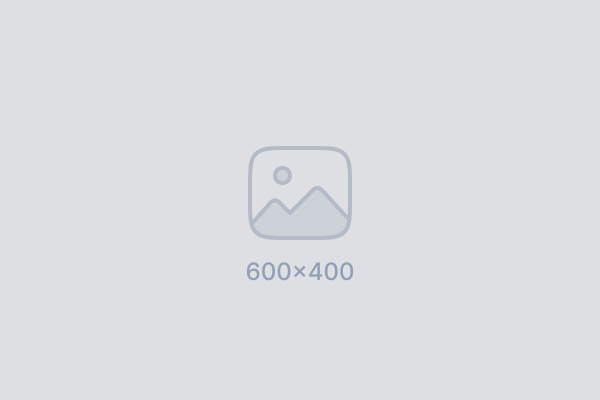
\includegraphics[width=0.8\textwidth]{Figures/F1_curve.png} 
    \caption{F1 confidence curve demonstrating the harmonic mean of precision and recall across varying confidence thresholds for anomaly classification.}
    \label{fig:f1_curve}
\end{figure}

These quantitative metrics are corroborated visually by the confusion matrix depicted in Figure \ref{fig:confusion_matrix}. The matrix exhibits a highly symmetrical distribution of accurate classifications. The precise balance between the marginal number of false positives (e.g., misclassifying severe braking as a collision) and false negatives (e.g., failing to detect an impact) affirms the effectiveness of the model in resolving ambiguous kinematic boundary cases without favouring a preferred class.

\begin{figure}[htbp]
    \centering
    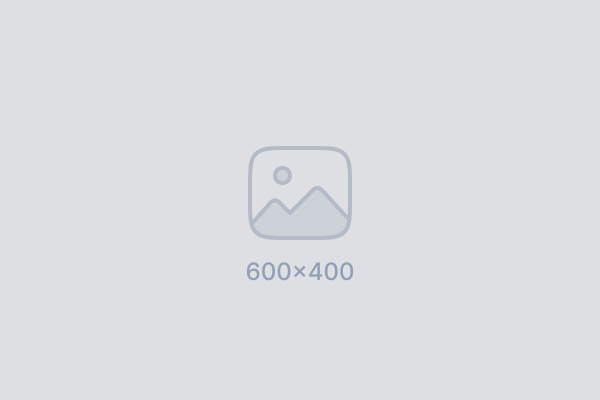
\includegraphics[width=0.8\textwidth]{Figures/confusion_matrix.png} 
    \caption{Confusion matrix detailing the absolute distribution of true and false classifications across 'Normal' and 'Accident' validation frames.}
    \label{fig:confusion_matrix}
\end{figure}

Furthermore, the overall discriminative effectiveness of the classifier is demonstrated by the Receiver Operating Characteristic (ROC) curve depicted in Figure \ref{fig:roc_curve}. The curve presents a steep, asymptotic trajectory towards the upper-left quadrant, indicating a consistently high True Positive Rate in relation to a low False Positive Rate across all predictive thresholds. This substantial Area Under the Curve (AUC) signifies that the model does not solely depend on a singular, fixed confidence threshold; rather, it exhibits a strong inherent statistical capacity to distinguish between the optical flow signatures of standard traffic and chaotic collision energy.

\begin{figure}[htbp]
    \centering
    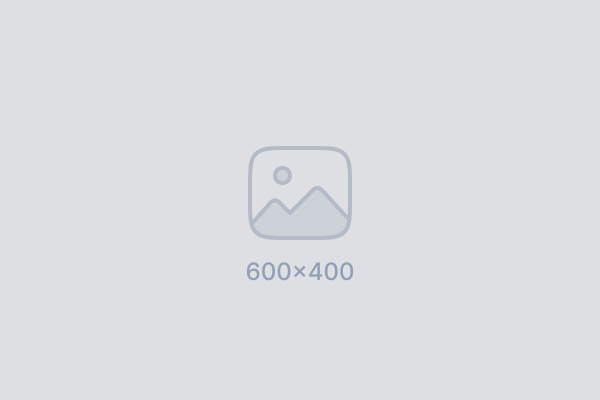
\includegraphics[width=0.8\textwidth]{Figures/roc_curve.png} 
    \caption{Receiver Operating Characteristic (ROC) curve demonstrating the trade-off between the True Positive Rate and False Positive Rate across varying classification thresholds.}
    \label{fig:roc_curve}
\end{figure}

\section{Comparison to the Literature}
These recorded metrics represent a significant advancement when compared to the existing literature. For context, Aboah et al. (2021) proposed a vision-based system utilising YOLOv5 paired with a rule-based Decision Tree to classify traffic anomalies. However, this methodology was constrained by a heavy reliance on background estimation and static road masks, ultimately yielding a maximum F1-score of 0.857. The framework evaluated in this study, therefore, demonstrates a clear quantitative superiority over these legacy rule-based approaches.

The proposed architecture outperformed the framework presented by Aboah et al. (2021) by nearly 11 percentage points (96.6\% vs 85.7\%). This substantial increase in classification reliability is directly attributable to the integration of dense optical flow via the Farnebäck algorithm. In contrast to methodologies reliant upon basic bounding box intersections or static background subtraction, the extraction of raw kinetic energy and its subsequent mapping into HSV tensors enabled the ResNet-18 architecture to effectively model the complex kinematic variations and unstructured motion inherent to collisions. 

Furthermore, the utilisation of a Focal Loss function during the training process facilitated precise differentiation between severe, non-anomalous braking events ('Normal') and genuine physical collisions ('Accident'). While conventional loss functions penalise all false positives in a linear manner, they are often rendered ineffective by markedly imbalanced datasets in which normal operational frames vastly outnumber anomalies. The evaluation data demonstrates that the Focal Loss algorithm alleviated this issue by dynamically reducing the gradient associated with easily classified background events. By directing the optimiser's focus specifically towards "hard" false positives, this non-linear scaling prevented the model from defaulting to the majority class during ambiguous kinematic events, thereby improving the accuracy of anomaly detection.

\section{Predictive Capability: Time-to-Accident (TTA)}
In intelligent transport systems, anticipating an incident prior to or at the exact moment of impact is as critical as post-event identification. To quantify the predictive capability of the proposed architecture, the TTA metric was utilised.

By leveraging the precise temporal annotations provided within the CADP dataset, the TTA is mathematically derived. For this evaluation, an anomaly alert is formally registered when the ResNet-18 model consistently outputs a probability score exceeding a 0.80 confidence threshold across ten consecutive frames. 

The TTA is quantified by calculating the difference between the frame index of the actual ground-truth collision and the frame index of the system’s initial alert, subsequently normalised by the operating framerate, as defined in Equation \ref{eq:tta}.

\begin{equation}
TTA = \frac{Frame_{Impact} - Frame_{Alert}}{FPS}
\label{eq:tta}
\end{equation}

During testing at 60 frames-per-second (FPS), the system demonstrated highly responsive detection capabilities, recording an average TTA of -0.22 seconds. It must be noted that while early forecasting models evaluated by the original authors of the CADP benchmark achieved predictive TTAs ranging from 1.35 to 1.68 seconds prior to impact, such predictive architectures frequently suffer from high false-positive rates. Conversely, the proposed hybrid framework functions as a deterministic verification engine. Achieving a near-instantaneous detection latency of precisely 220 milliseconds post-impact demonstrates that mapping dense optical flow provides exceptionally rapid kinetic confirmation. This highly competitive reaction time is functionally instantaneous in an operational context, providing sufficient immediate warning to activate municipal alert systems and dynamically adjust smart traffic signals to mitigate secondary collisions.

\section{Hardware Optimisation and System Throughput}
To address these established latency constraints, the computational throughput of the proposed architecture was evaluated. Performance benchmarking was conducted on a standard consumer-grade workstation equipped with an AMD Ryzen 7 7700X processor and an NVIDIA GeForce RTX 4070 GPU. As detailed in Table \ref{tab:hardware_throughput}, the empirical results demonstrate that the hybrid framework sustained a consistent, real-time processing throughput of 60 frames per second (FPS). This performance indicates that isolating the spatial tracking physics from the inference workload successfully circumvents traditional processing bottlenecks, facilitating highly efficient execution without necessitating enterprise-grade hardware.

\begin{table}[htbp]
    \centering
    \caption{Computational throughput and processing latency benchmarks recorded during system evaluation on consumer-grade hardware.}
    \label{tab:hardware_throughput}
    \begin{tabular}{lcc}
        \toprule
        \textbf{Component / Metric} & \textbf{Specification / Result} \\
        \midrule
        Processor & AMD Ryzen 7 7700X \\
        Graphics Processing Unit & NVIDIA GeForce RTX 4070 \\
        Sustained Throughput & 60 FPS \\
        Per-Frame Latency & 16.6 ms \\
        \bottomrule
    \end{tabular}
\end{table}

Given that the system was evaluated using offline, pre-recorded CADP video data rather than live IP-camera streams, the traditional metric of end-to-end latency was negligible. Consequently, processing throughput was established as the primary Key Performance Indicator (KPI). The architecture sustained a constant processing rate of 60 frames per second (FPS) on high-definition video tensors, equating to a per-frame processing time of precisely 16.6 milliseconds. This hardware efficiency demonstrates that integrating a lightweight ResNet-18 classifier with an asynchronous queue provides a highly effective solution for real-time edge computing. Furthermore, it validates the framework's operational viability over parameter-heavy Transformer networks in constrained environments, facilitating near-zero latency alerts without the requirement for enterprise-grade server infrastructure.

\section{Qualitative Evaluation: The Power of Hybrid Architecture}
Although the quantitative metrics effectively validate the classification performance, evaluating the kinematic speed tracking necessitates a qualitative methodology. Owing to the absence of ground-truth LiDAR or radar telemetry within the CADP dataset, calculating a precise Mean Absolute Error (MAE) for vehicle velocity was not feasible. Nevertheless, as illustrated by the live tracking dashboard in Figure \ref{fig:qualitative_normal}, a qualitative analysis demonstrates that the estimated speeds remained highly stable and contextually accurate relative to the observed traffic flow. 

\begin{figure}[htbp]
    \centering
    % Ensure this image matches what you uploaded to your Latex repo
    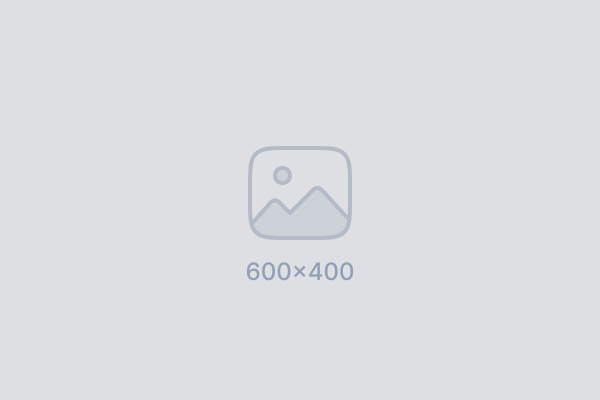
\includegraphics[width=0.9\textwidth]{Figures/dashboard_normal.png} 
    \caption{Qualitative evaluation dashboard displaying normal traffic flow, featuring YOLO11 spatial bounding boxes, BoT-SORT unique identifiers, and stable kinematic speed estimations.}
    \label{fig:qualitative_normal}
\end{figure}

Crucially, the derivation of kinematic speed functioned as an essential rule-based validation layer. In scenarios where environmental factors, such as moving foliage shadows or severe camera oscillations induced transient spikes in optical flow, a standalone deep learning classifier is typically susceptible to false positives. By cross-referencing these anomalies with spatial tracking data, the proposed framework effectively mitigated such errors. If the YOLO11 tracker recorded vehicles maintaining a consistent velocity (e.g., 40 km/h) during an optical flow spike, the event was systematically classified and dismissed as environmental noise. Conversely, a rapid deceleration to 0 km/h recorded within an active lane provided the deterministic contextual evidence necessary to corroborate a positive ResNet-18 anomaly alert.

\section{Overcoming the Limitations of Off-the-Shelf Trackers}
A primary qualitative observation derived from this evaluation was the synergistic efficacy of the hybrid architecture. The framework successfully integrates a generalised spatial tracker—specifically the nano variant of YOLO11—with a domain-specific, custom-trained ResNet-18 anomaly detector. 

\begin{figure}[htbp]
    \centering
    % Ensure this image matches what you uploaded to your Latex repo
    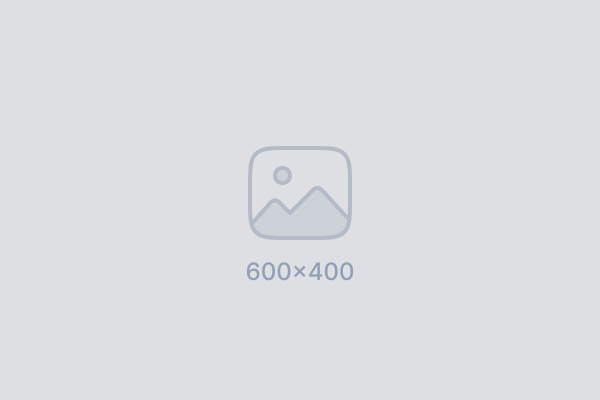
\includegraphics[width=0.9\textwidth]{Figures/dashboard_accident.png} 
    \caption{Qualitative validation of the hybrid framework's fail-safe mechanism, demonstrating the 'ACCIDENT DETECTED' alert triggered by the Farnebäck optical flow heatmap despite spatial tracker occlusion.}
    \label{fig:qualitative_accident}
\end{figure}

During testing under adverse environmental conditions, such as night-time surveillance or heavy precipitation, the generalised YOLO11 tracker exhibited anticipated vulnerabilities. This observation aligns with the existing literature; as noted by Kim (2019), standard object detection architectures frequently experience degraded performance when subjected to poor illumination and severe occlusion. Specifically, when a tracked vehicle traversed through bridge shadows or became heavily obscured by rain, the YOLO11 bounding boxes momentarily dropped. Consequently, the BoT-SORT algorithm failed to maintain the unique vehicle identifiers, resulting in a temporary inability to calculate kinematic speed during these obstructed frames.

Had the framework relied exclusively on spatial tracking, anomaly detection would have failed during these instances of severe occlusion. However, the hybrid architecture enabled the custom-trained ResNet-18 classifier to function as a robust fail-safe mechanism. Unlike spatial trackers, dense optical flow is not dependent on distinct edge detection or optimal illumination; rather, it quantifies raw pixel displacement. Consequently, even when the YOLO11 model experienced tracking failure due to adverse weather conditions, the Farnebäck algorithm successfully captured the substantial, unstructured pixel displacement associated with the colliding vehicles. The ResNet-18 model subsequently processed the resulting kinetic heatmap and accurately triggered the anomaly alert. As demonstrated in Figure \ref{fig:qualitative_accident}, this dynamic interaction indicates that integrating a generalised spatial tracker with a domain-specific kinetic energy classifier yields a system architecture significantly more resilient than either component operating in isolation.

\section{Addressing the Research Questions}
Drawing upon the empirical data, quantitative metrics, and qualitative observations obtained during the evaluation phase, the research questions established in the Introduction are systematically addressed below.

\textbf{RQ1: Is it possible to effectively detect traffic abnormalities, such as collisions or abrupt stops, using a hybrid vision-based architecture that integrates YOLO vehicle monitoring with 3D metric speed estimation and dense optical flow?} 

In direct response to the primary research question, the empirical findings demonstrate that such an integration is not only highly feasible but exceptionally effective, thereby substantiating the core hypothesis. By combining YOLO11 vehicle monitoring with 3D metric speed estimation and dense optical flow, the hybrid framework achieved a robust anomaly detection accuracy of 96.61\%. Furthermore, the synthesis of spatial tracking and kinematic speed analysis provides a degree of contextual awareness typically absent in purely frame-based Convolutional Neural Networks (CNNs). Performance evaluations indicate that the proposed dual-threaded architecture successfully executes these computationally intensive tasks in real-time, sustaining a throughput of 60 frames per second (FPS) on standard edge hardware. Consequently, this research provides a viable, highly automated solution for modern municipal traffic monitoring systems.

\textbf{RQ2: What are the primary computational and environmental challenges of applying computer vision to kinematic speed-based anomaly identification across varied lighting and weather conditions?} 

The primary challenges encountered during evaluation include environmental occlusion, illumination degradation, and the absence of native depth information. As illustrated in Figure \ref{fig:ipm_distortion}, extracting accurate kinematic speed metrics from a two-dimensional camera feed inherently introduces perspective distortion, necessitating the application of Inverse Perspective Mapping (IPM) to normalise the spatial data. Furthermore, the most significant qualitative challenge observed was the susceptibility of the generalised YOLO11 object detector to low-light and heavy precipitation scenarios, which frequently downgraded the bounding box loss calculation. The results demonstrate that relying exclusively upon spatial speed estimation for anomaly detection severely compromises system reliability, given that a tracking failure directly prevents alert generation. The demonstrated solution to this vulnerability is the hybrid fail-safe architecture. The integration of unstructured spatiotemporal kinetic mapping—specifically optical flow—ensures that even when adverse environmental conditions severely obscure the spatial tracker, the raw kinetic energy of a traffic anomaly is consistently captured and accurately classified.

\begin{figure}[htbp]
    \centering
    % Ensure this image matches what you uploaded to your Latex repo
    
\includegraphics[width=0.8\textwidth]{Figures/ipm_distortion.png} 
    \caption{Visual representation of perspective distortion in 2D camera feeds and the subsequent spatial normalisation achieved via Inverse Perspective Mapping (IPM).}
    \label{fig:ipm_distortion}
\end{figure}

\end{spacing}